\documentclass[crop,tikz]{standalone}% 'crop' is the default for v1.0, before it was 'preview'
\usepackage{pgfplots}
\usetikzlibrary{math}
\begin{document}
    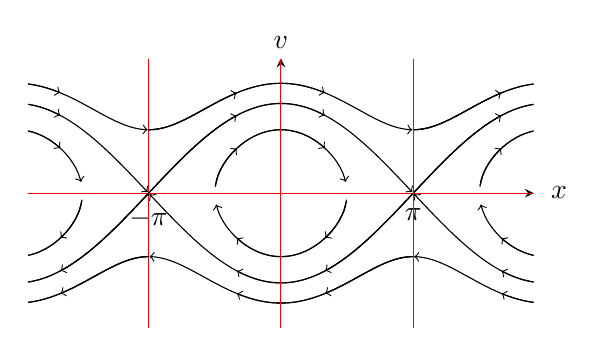
\begin{tikzpicture}
  	\tikzmath{\xa = 6; \y = 3;}
	\begin{axis}[
	    width=8cm,
	    height=5cm,
	    xmin= -\xa, xmax= \xa,
	    ymin= -\y, ymax = \y,
	    axis lines = middle,
	    x label style={at={(axis description cs:1.05,0.56)},anchor=north},
	    y label style={at={(axis description cs:0.5,1)},anchor=south},
	    xlabel={$x$},
	    ylabel={$v$},
	    xtick={0, pi, -pi},
	    xticklabels={$0$, $\pi$, $-\pi$},
	    ytick={0},
	    yticklabel={},
	    ]
	    %%%%%%%%%%%%%%%%%%%%%%%%%%%%%%%%%%%
	    %  Linea orizzontale (nurk line)  %
	    %%%%%%%%%%%%%%%%%%%%%%%%%%%%%%%%%%%
	    \addplot [domain=-\xa:\xa, samples=5, red] {0};
	    
	    \foreach \n in {-2*pi,0,2*pi} { % Vario "l'occhio" da visualizzare
		\foreach \s in {0.01,1,2} { % Traccio più linee per avere più punte di freccia
		    \foreach \E in {-1, 0 , 1} { % Vario l'energia per vedere le tre aree dello spazio delle fasi
			%%%%%%%%%%%%%%%%%%%%%%%%%%%%%%%%%%%%%%%%%%%%%
			%  Linee del moto al variare della energia  %
			%%%%%%%%%%%%%%%%%%%%%%%%%%%%%%%%%%%%%%%%%%%%%
		    	\addplot [domain= ( -pi-\n): ( pi-\n ) - 2*pi*\s/3, samples=100, ->] {sqrt( 2*(\E + 1 + cos(deg(x)) ))};
		    	\addplot [domain= ( -pi-\n) + 2*pi*\s/3: ( pi-\n ) , samples=100, <-] {-sqrt( 2*(\E + 1 + cos(deg(x)) ))};
		    }
		}
		%%%%%%%%%%%%%%%%%%%%%%%%%%%%%%%%%%
		%  Linee verticali (nurk lines)  %
		%%%%%%%%%%%%%%%%%%%%%%%%%%%%%%%%%%
	    	\addplot [red] coordinates {(\n/2, -\y) (\n/2, \y)};
	    }
	\end{axis}
    \end{tikzpicture}
\end{document}
